\subsubsection{API Gateway}

L'API Gateway è il cuore della piattaforma. Il suo compito è, previa verifica dei privilegi e aggiornamento del database SLA, reindirizzare le chiamate dell'utilizzatore finale e instradarle verso il fornitore del microservizio. La necessità del passaggio per un gateway centralizzato è per motivi di data analysis, nonchè di controllo della validità delle chiavi. \\
L'API Gateway è un package del back-end, tuttavia, l'approccio a microservizi adottato, ci consente di descriverlo come un'entità a sè stante. Esso è composto dai campi dati, per mantenere in coda le chiamate, e un servizio interno, che si occupa di effettuare le operazioni di verifica chiave, verifica e scrittura SLA, forwarding delle chiamate e forwarding delle risposte.  \\
Il package principale per il servizio API Gateway è rappresentato dal seguente diagramma UML:

\begin{figure}[H]
	\centering
	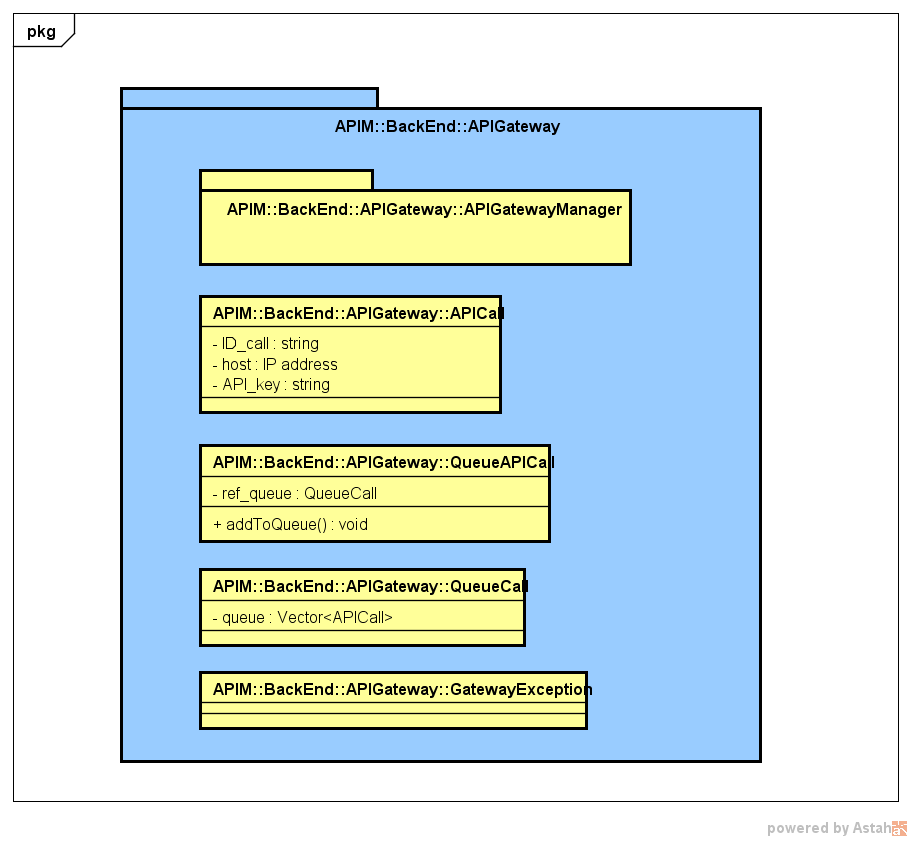
\includegraphics[scale=0.45]{UML/DiagrammiPackage/APIGateway.png}
	\caption{Package APIM::BackEnd::APIGateway}
\end{figure}


Il package \textit{APIGateway}, che rappresenta il servizio omonimo, contiene il seguente package:

\begin{itemize}
	\item \textbf{APIGatewayManager}: questo package si occupa di gestire le richieste in arrivo, instradare la richiesta al microservizio richiesto e di ovviare, in modo opportuno, alle condizioni di errore.
\end{itemize}

\paragraph{APICall}
\begin{itemize}
	\item \textbf{Funzione del componente}: la classe si occuper\`{a} di istanziare un oggetto che rappresenta la chiamata a un microservizio ricevuta da un client, che verrà poi inserita in \textit{QueueAPICall};
	\item \textbf{Relazioni d'uso di altri componenti}: \textit{QueueAPICall};
	\item \textbf{Attività svolte e dati trattati}: la classe contiene un id che identifica univocamente una chiamata, un indirizzo IP per sapere dove restituire la risposta della chiamata e la API key dell'utente.
\end{itemize}

\paragraph{QueueAPICall}
\begin{itemize}
	\item \textbf{Funzione del componente}: questa classe istanzier\`{a} un numero finito di oggetti, di numero controllato, in modo da garantire un buon servizio, che conterr\`{a} una struttura dati Vector, usata per contenere le \textit{APICall};
	\item \textbf{Relazioni d'uso di altri componenti}: \textit{APICall};
	\item \textbf{Attività svolte e dati trattati}: il suo compito principale sar\`{a} registrare la richiesta a un microservizio.
\end{itemize}

\paragraph{GatewayException}
\begin{itemize}
	\item \textbf{Funzione del componente}: questa classe istanzier\`{a} un oggetto che rappresenta una condizione d'errore nella richiesta ricevuta;
	\item \textbf{Relazioni d'uso di altri componenti}: \textit{APICall}.
\end{itemize}

\paragraph{APIGatewayManager}
\begin{figure}[H]
	\centering
	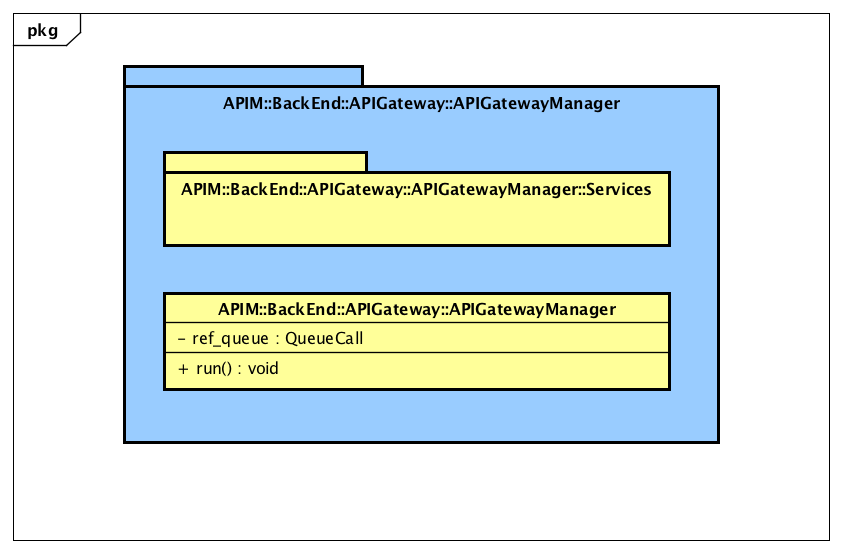
\includegraphics[scale=0.45]{UML/DiagrammiPackage/APIGatewayManager.png}
	\caption{Package APIM::BackEnd::APIGateway::APIGatewayManager}
\end{figure}

Il package \textit{APIGatewayManager}, che rappresenta il servizio omonimo, contiene il seguente package:
\begin{itemize}
	\item \textbf{Services}: questo package si occupa di gestire le funzionalità di controllo e verifica delle chiamate ai microservizi, che passano per l'API Gateway.
\end{itemize}

\subparagraph{APIGatewayManager}
\begin{itemize}
	\item \textbf{Funzione del componente}: questa classe istanzier\`{a} un oggetto che rappresenta un task, il quale avr\`{a} il compito di avviare un thread che gestir\`{a} le richieste correnti all'APIGateway, immagazzinate in \textit{QueueAPICall}, mediante i servizi forniti. Inoltre, salverà i dati della chiamata correntemente eseguita in \textit{Buffer}, così da averli a disposizione per l'elaborazione;
	\item \textbf{Relazioni d'uso di altri componenti}: \textit{QueueAPICall}, \textit{Buffer}, \textit{Verifier}, \textit{SLALogger}, \textit{RequestForwarder}, \textit{ResponseForwarder}.
\end{itemize}

\subparagraph{Services}
\begin{figure}[H]
	\centering
	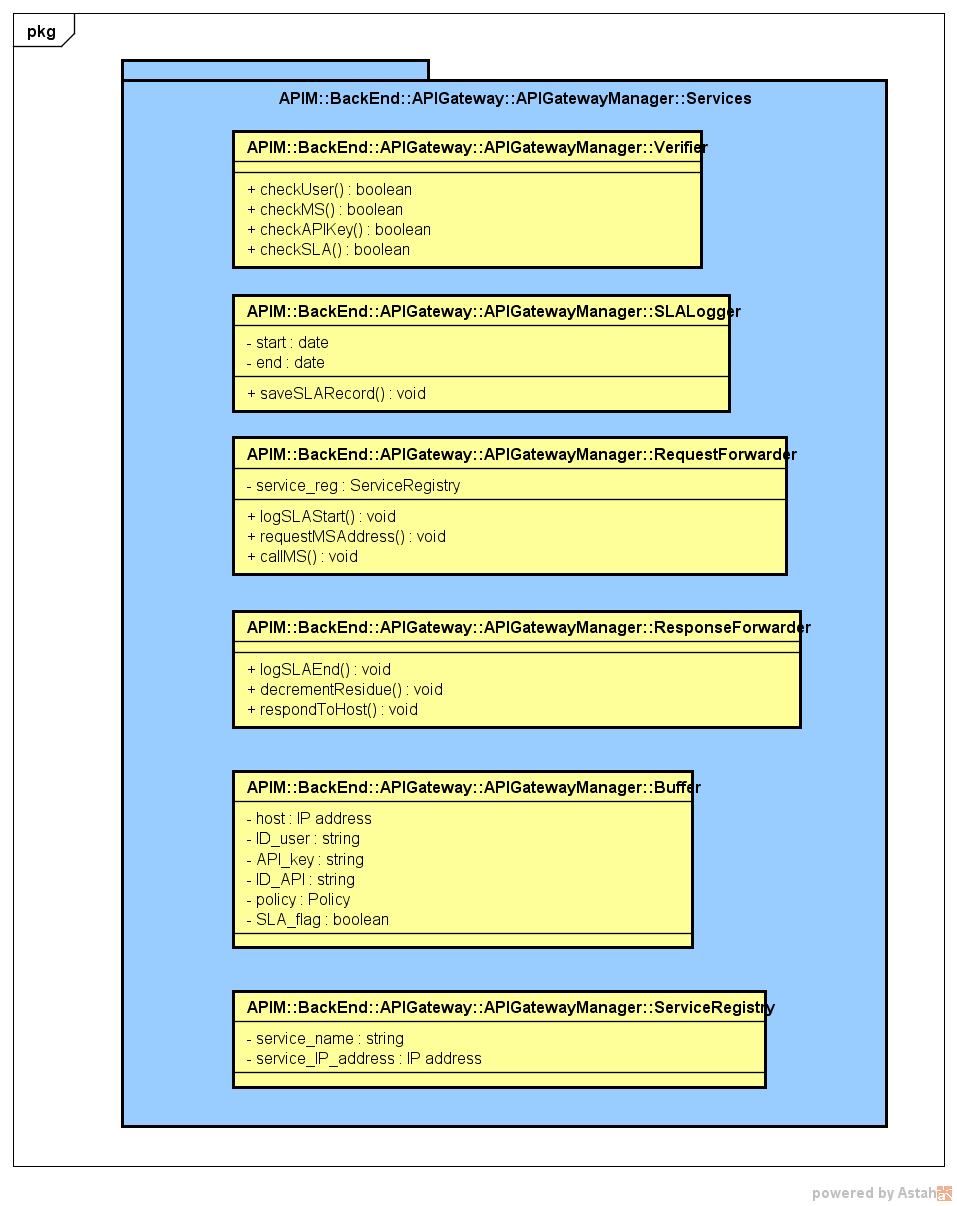
\includegraphics[scale=0.45]{UML/DiagrammiPackage/APIGatewayManagerServices.png}
	\caption{Package APIM::BackEnd::APIGateway::APIGatewayManager::Services}
\end{figure}
\FloatBarrier

\chapter{\textbf{Verifier}}
\begin{itemize}
	\item \textbf{Funzione del componente}: la classe rappresenta un microservizio che si occupa di verificare che la richiesta ricevuta all'API Gateway sia valida;
	\item \textbf{Relazioni d'uso di altri componenti}: \textit{RequestForwarder};
	\item \textbf{Attivit\`{a} svolte e dati trattati}: la classe controller\`{a} che l'utente sia un utente valido, che il microservizio esista e sia attivo, che l'API key dell'utente non sia scaduta e che la SLA associata alla richiesta sia rispettata.
\end{itemize}

\chapter{\textbf{SLALogger}}
\begin{itemize}
	\item \textbf{Funzione del componente}: la classe si occuper\`{a} di istanziare un oggetto che rappresenta gli intervalli di inizio e fine di una chiamata a un microservizio;
	\item \textbf{Relazioni d'uso di altri componenti}: \textit{RequestForwarder}, \textit{ResponseForwarder};
	\item \textbf{Attivit\`{a} svolte e dati trattati}:  la classe avr\`{a} il compito di salvare in un buffer la data di inizio e fine di una chiamata, sulla base dell'ID di quella chiamata, attraverso dei dati che ricever\`{a} dagli altri componenti dell'API Gateway.	
\end{itemize}

\chapter{\textbf{RequestForwarder}}
\begin{itemize}
	\item \textbf{Funzione del componente}: la classe si occuper\`{a} di istanziare un oggetto che avr\`{a} il compito di instradare la richiesta ricevuta al microservizio corretto e salvare i dati della richiesta;
		\item \textbf{Relazioni d'uso di altri componenti}: \textit{ServiceRegistry}, \textit{SLALogger};
		\item \textbf{Attivit\`{a} svolte e dati trattati}: la classe, sulla base delle informazioni dell'IP recuperato dal \textit{ServiceRegistry}, inoltrer\`{a} la richiesta ricevuta al microservizio corretto e richieder\`{a} allo \textit{SLALogger} di salvare i dati relativi al tempo di inizio della richiesta.
\end{itemize}

\chapter{\textbf{ResponseForwarder}}
\begin{itemize}
	\item \textbf{Funzione del componente}: la classe si occuper\`{a} di istanziare un oggetto che avr\`{a} il compito di ricevere la risposta da parte di un microservizio sulla base di una chiamata al microservizio e salvare i dati relativi alla richiesta;
	\item \textbf{Relazioni d'uso di altri componenti}: \textit{SLALogger};
	\item \textbf{Attivit\`{a} svolte e dati trattati}: comunica con lo \textit{SLALogger} per salvare i dati circa il tempo di fine della richiesta, o in caso di esito negativo della richiesta, di apporre il corretto flag per segnalarlo. Inoltra, poi, i dati di risposta al client richiedente.
\end{itemize}

\chapter{\textbf{Buffer}}
\begin{itemize}
	\item \textbf{Funzione del componente}: la classe si occuper\`{a} di istanziare una oggetto che rappresenta un buffer;
	\item \textbf{Attivit\`{a} svolte e dati trattati}: contiene l'IP dell'host, l'ID dell'utente che ha effettuato la richiesta, l'API Key e il relativo ID, la policy di vendita e un flag relativo alla SLA, per indicare se è rispettata o meno.
\end{itemize}

\chapter{\textbf{ServiceRegistry}}
\begin{itemize}
	\item \textbf{Funzione del componente}: la classe si occuper\`{a} di istanziare una classe oggetto che rappresenta un microservizio;
	\item \textbf{Relazioni d'uso di altri componenti}: \textit{RequestForwarder};
	\item \textbf{Attivit\`{a} svolte e dati trattati}: la classe fornisce le generalit\`{a} del microservizio (IP e nome).
\end{itemize}